\section{Evaluation}

\begin{figure}[h]
    \centering
    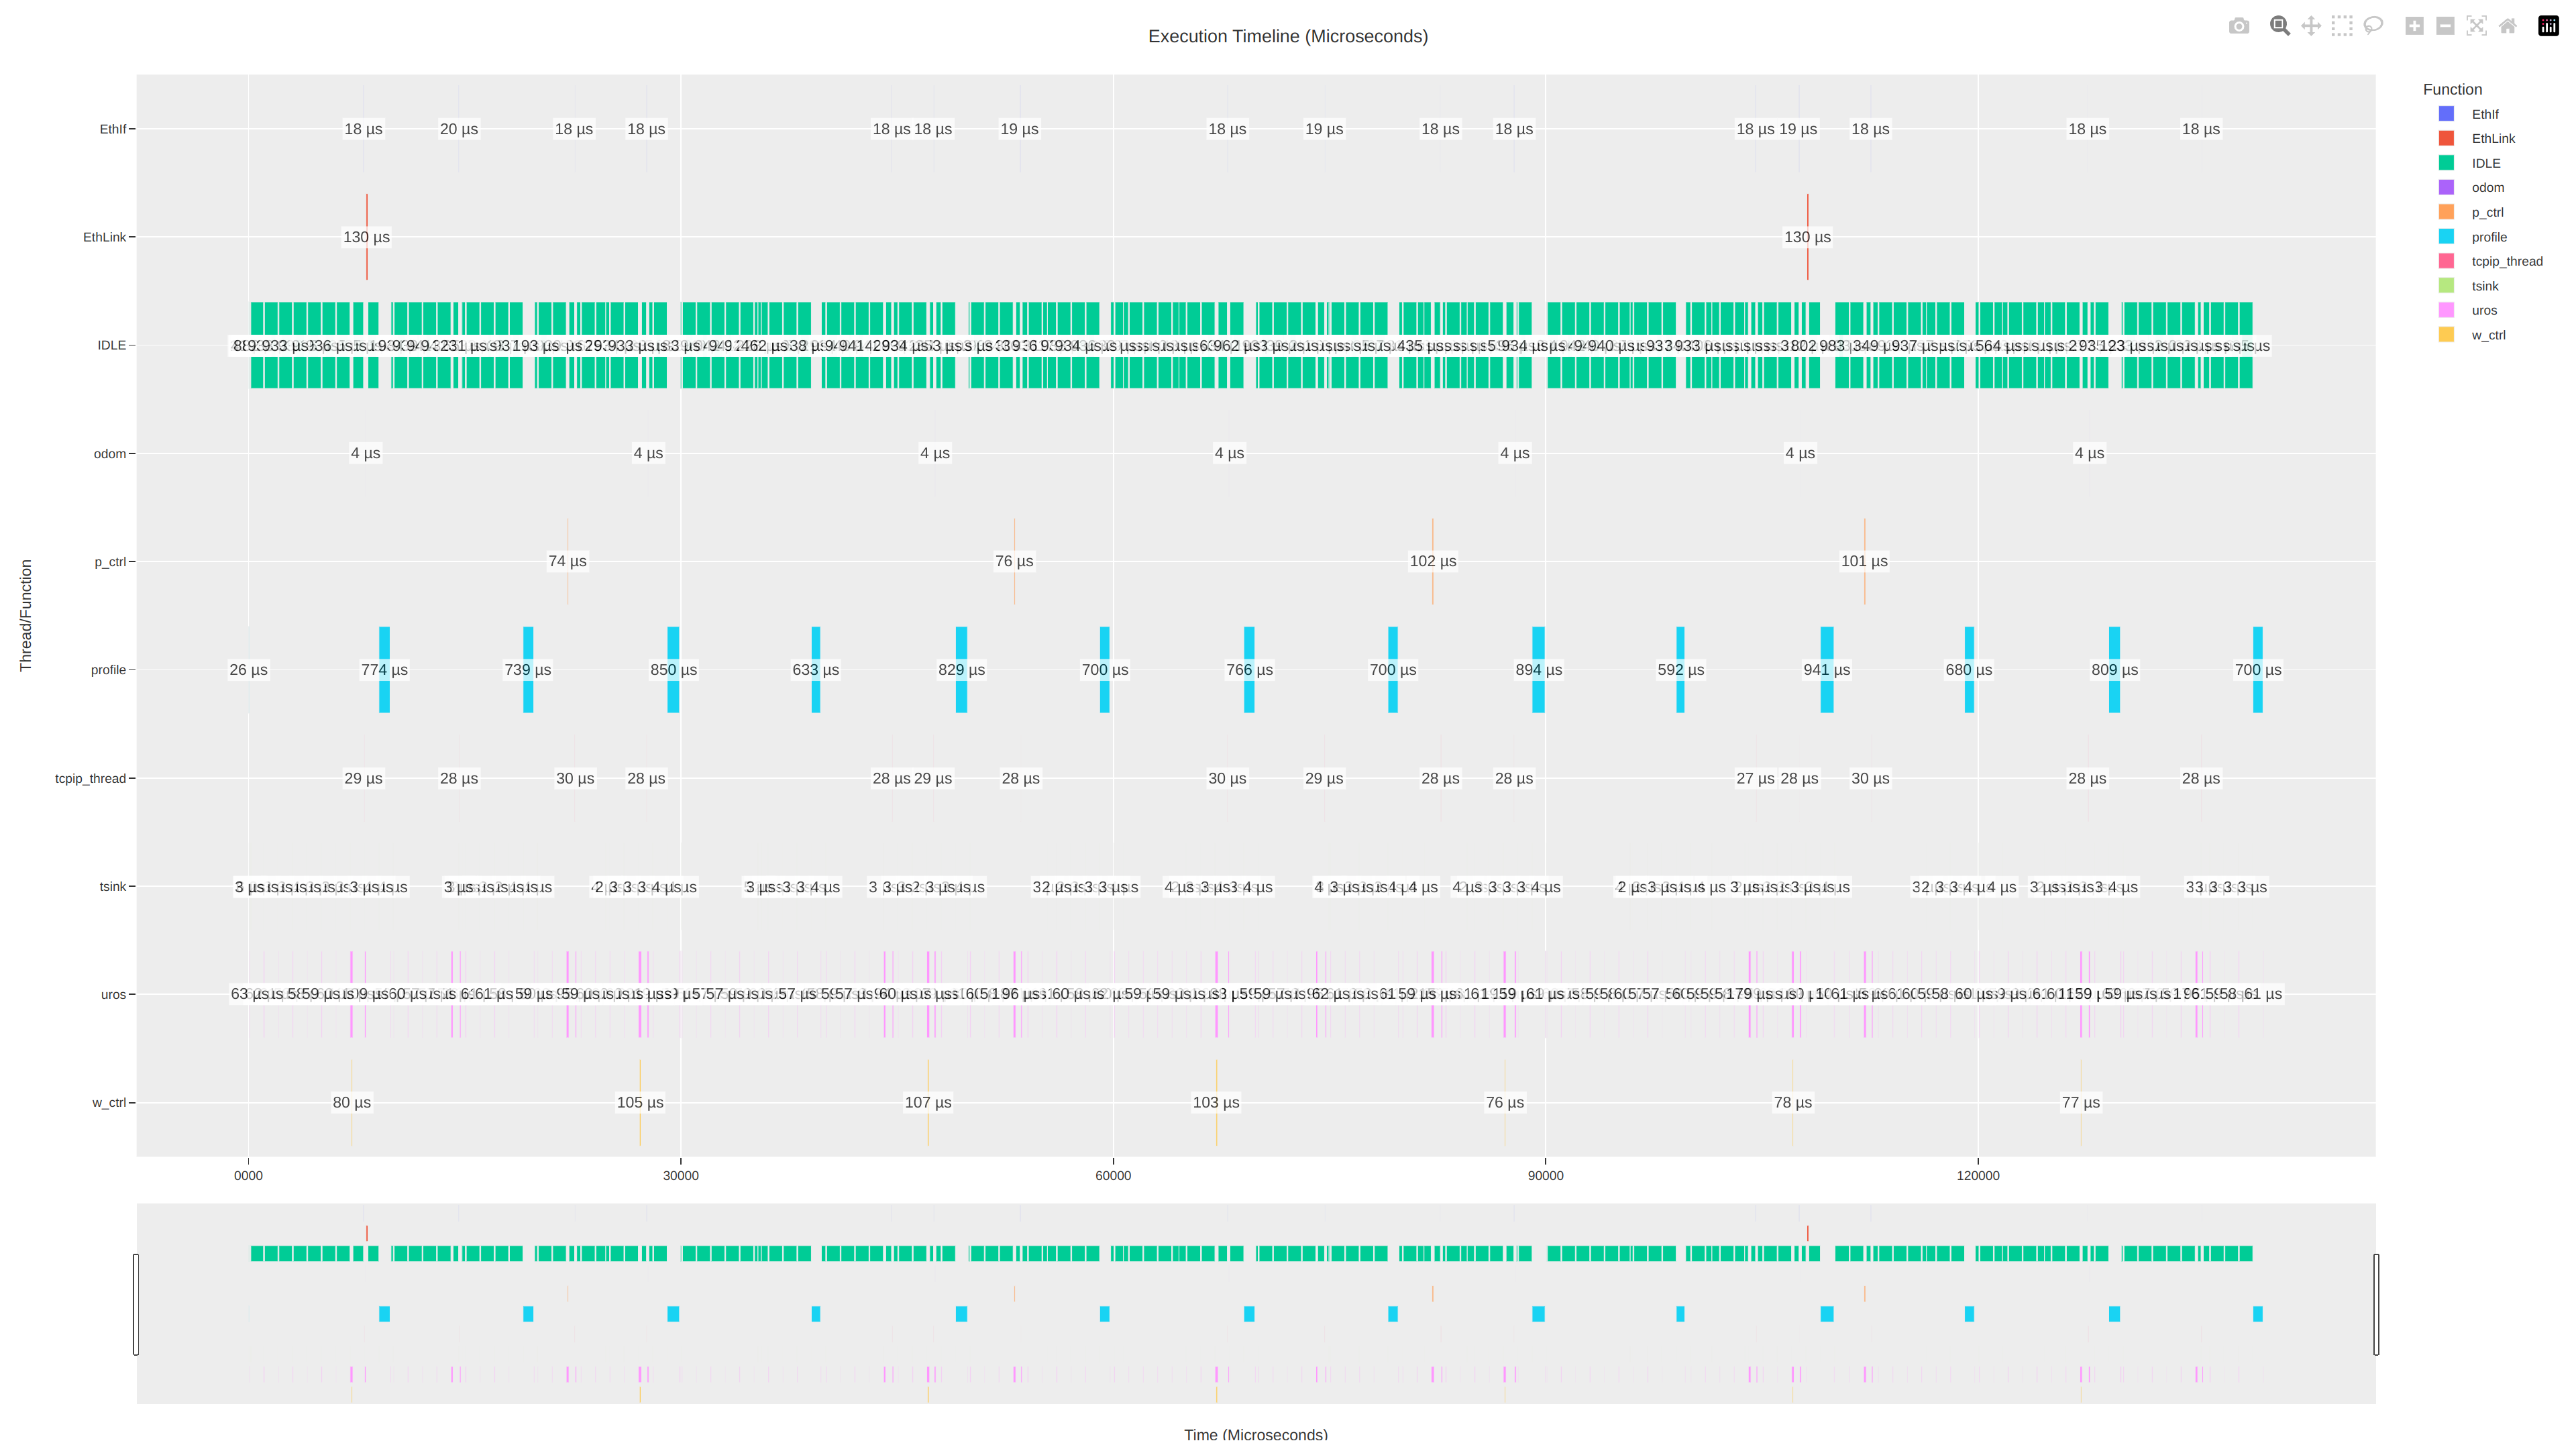
\includegraphics[width=1\textwidth]{assets/micro_ros_profiling}
    \caption{Visualisierung der Echtzeitanalyse unter Micro-ROS}
    % \label{fig:micro_ros_profiling}
\end{figure}

\begin{code}
\begin{minted}{cpp}
=======================================
free heap:          4688
ctx switches:       126810
Task            Time        %
profile         33450       2%
uros            106984      8%
IDLE            1179311     88%
EthLink         1695        <1%
tcpip_thread    4526        <1%
tsink           3762        <1%
Tmr Svc         0           <1%
EthIf           2730        <1%
---------------------------------------
Task        State   Prio    Stack   Num
uros            R     24     2548     3
profile         X     24     892      2
IDLE            R     0      108      4
tcpip_thread    B     24     180      6
tsink           B     32     475      1
EthLink         B     16     193      8
EthIf           B     48     17       7
Tmr Svc         B     2      223      5
=======================================
profiled for 18881864 us
\end{minted}
    \captionof{listing}{Zusammenfassung Echtzeitanalyse unter Micro-ROS}
\end{code}

\begin{figure}[h]
    \centering
    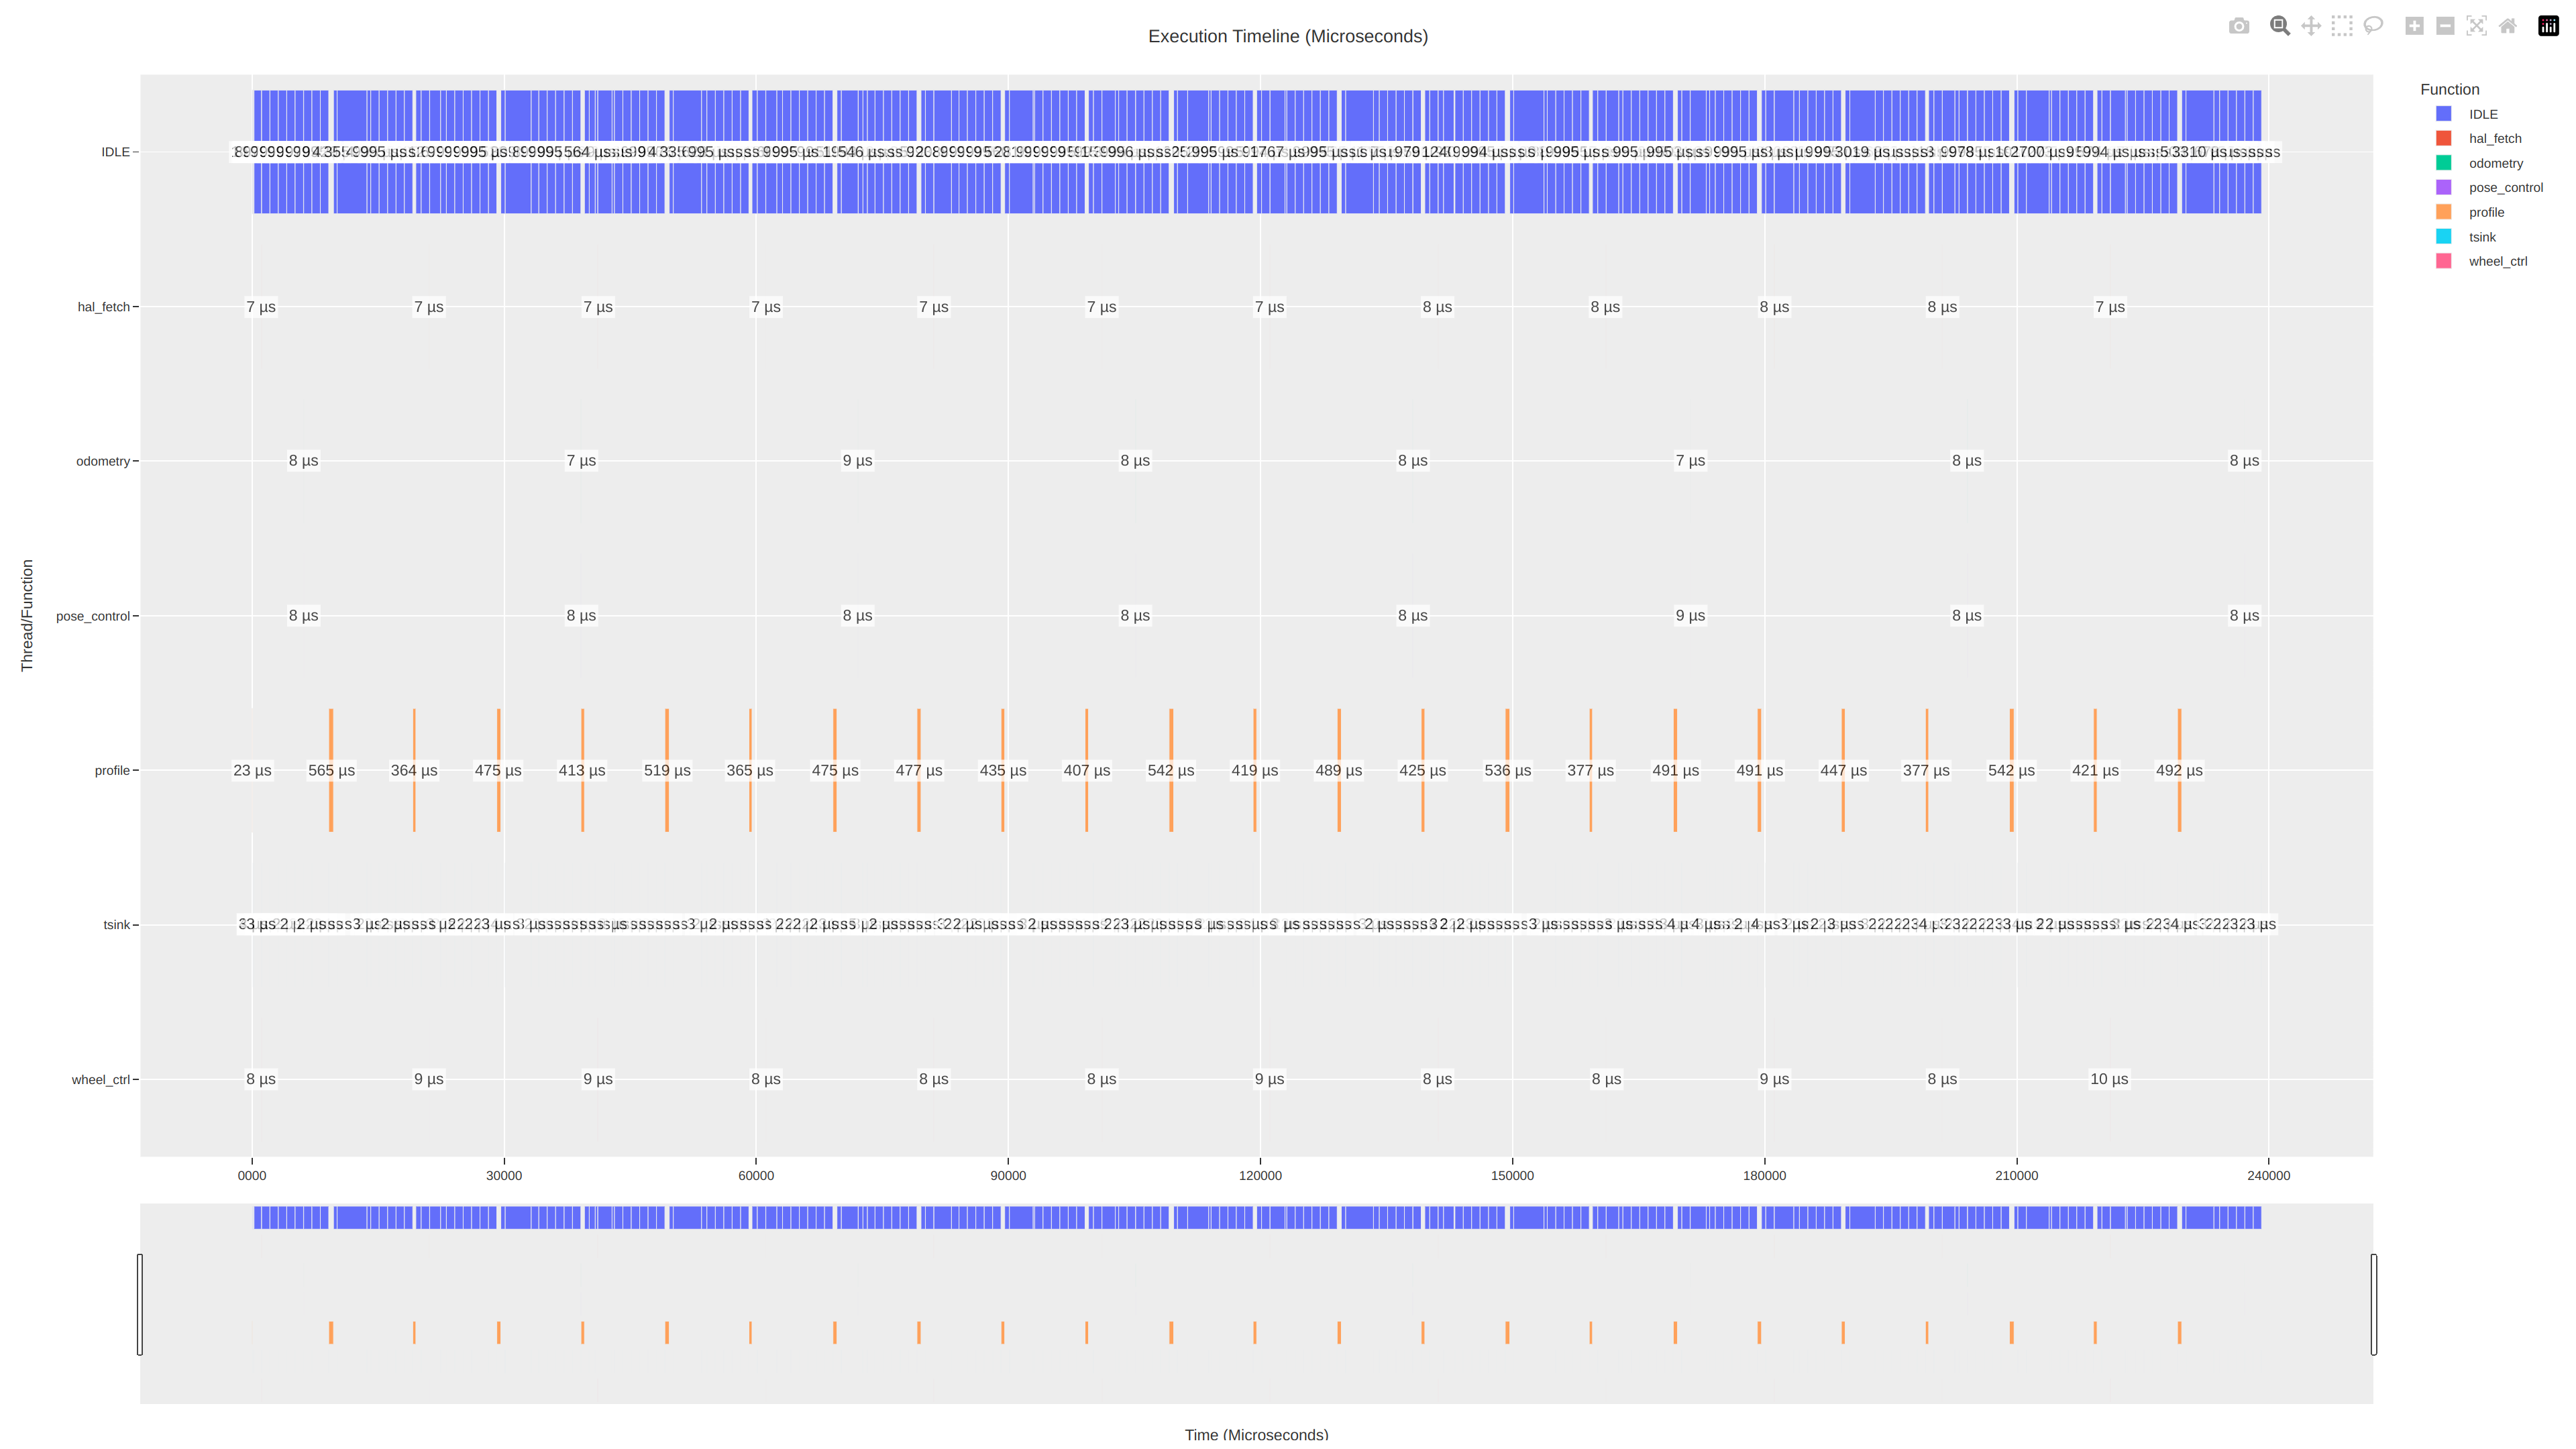
\includegraphics[width=1\textwidth]{assets/freertos_profiling}
    \caption{Visualisierung der Echtzeitanalyse unter FreeRTOS}
    % \label{fig:freertos_profiling}
\end{figure}

\begin{code}
\begin{minted}{cpp}
=======================================
free heap:          195696
ctx switches:       76148
Task            Time        %%
profile         9669        4%
IDLE            201086      95%
hal_fetch       81          <1%
wheel_ctrl      87          <1%
odometry        49          <1%
pose_control    51          <1%
tsink           615         <1%
Tmr Svc         0           <1%
recv_vel        0           <1%
---------------------------------------
Task        State   Prio    Stack   Num
profile         X      24     900     7
IDLE            R      0      108     8
wheel_ctrl      B      24     420     5
odometry        B      24     416     6
pose_control    B      24     410     4
tsink           B      32     483     1
hal_fetch       B      24     443     2
recv_vel        S      24     441     3
Tmr Svc         B      2      223     9
=======================================
profiled for 18779120 us
\end{minted}
    \captionof{listing}{Zusammenfassung Echtzeitanalyse unter Micro-ROS}
\end{code}

\begin{figure}[h]
    \centering
    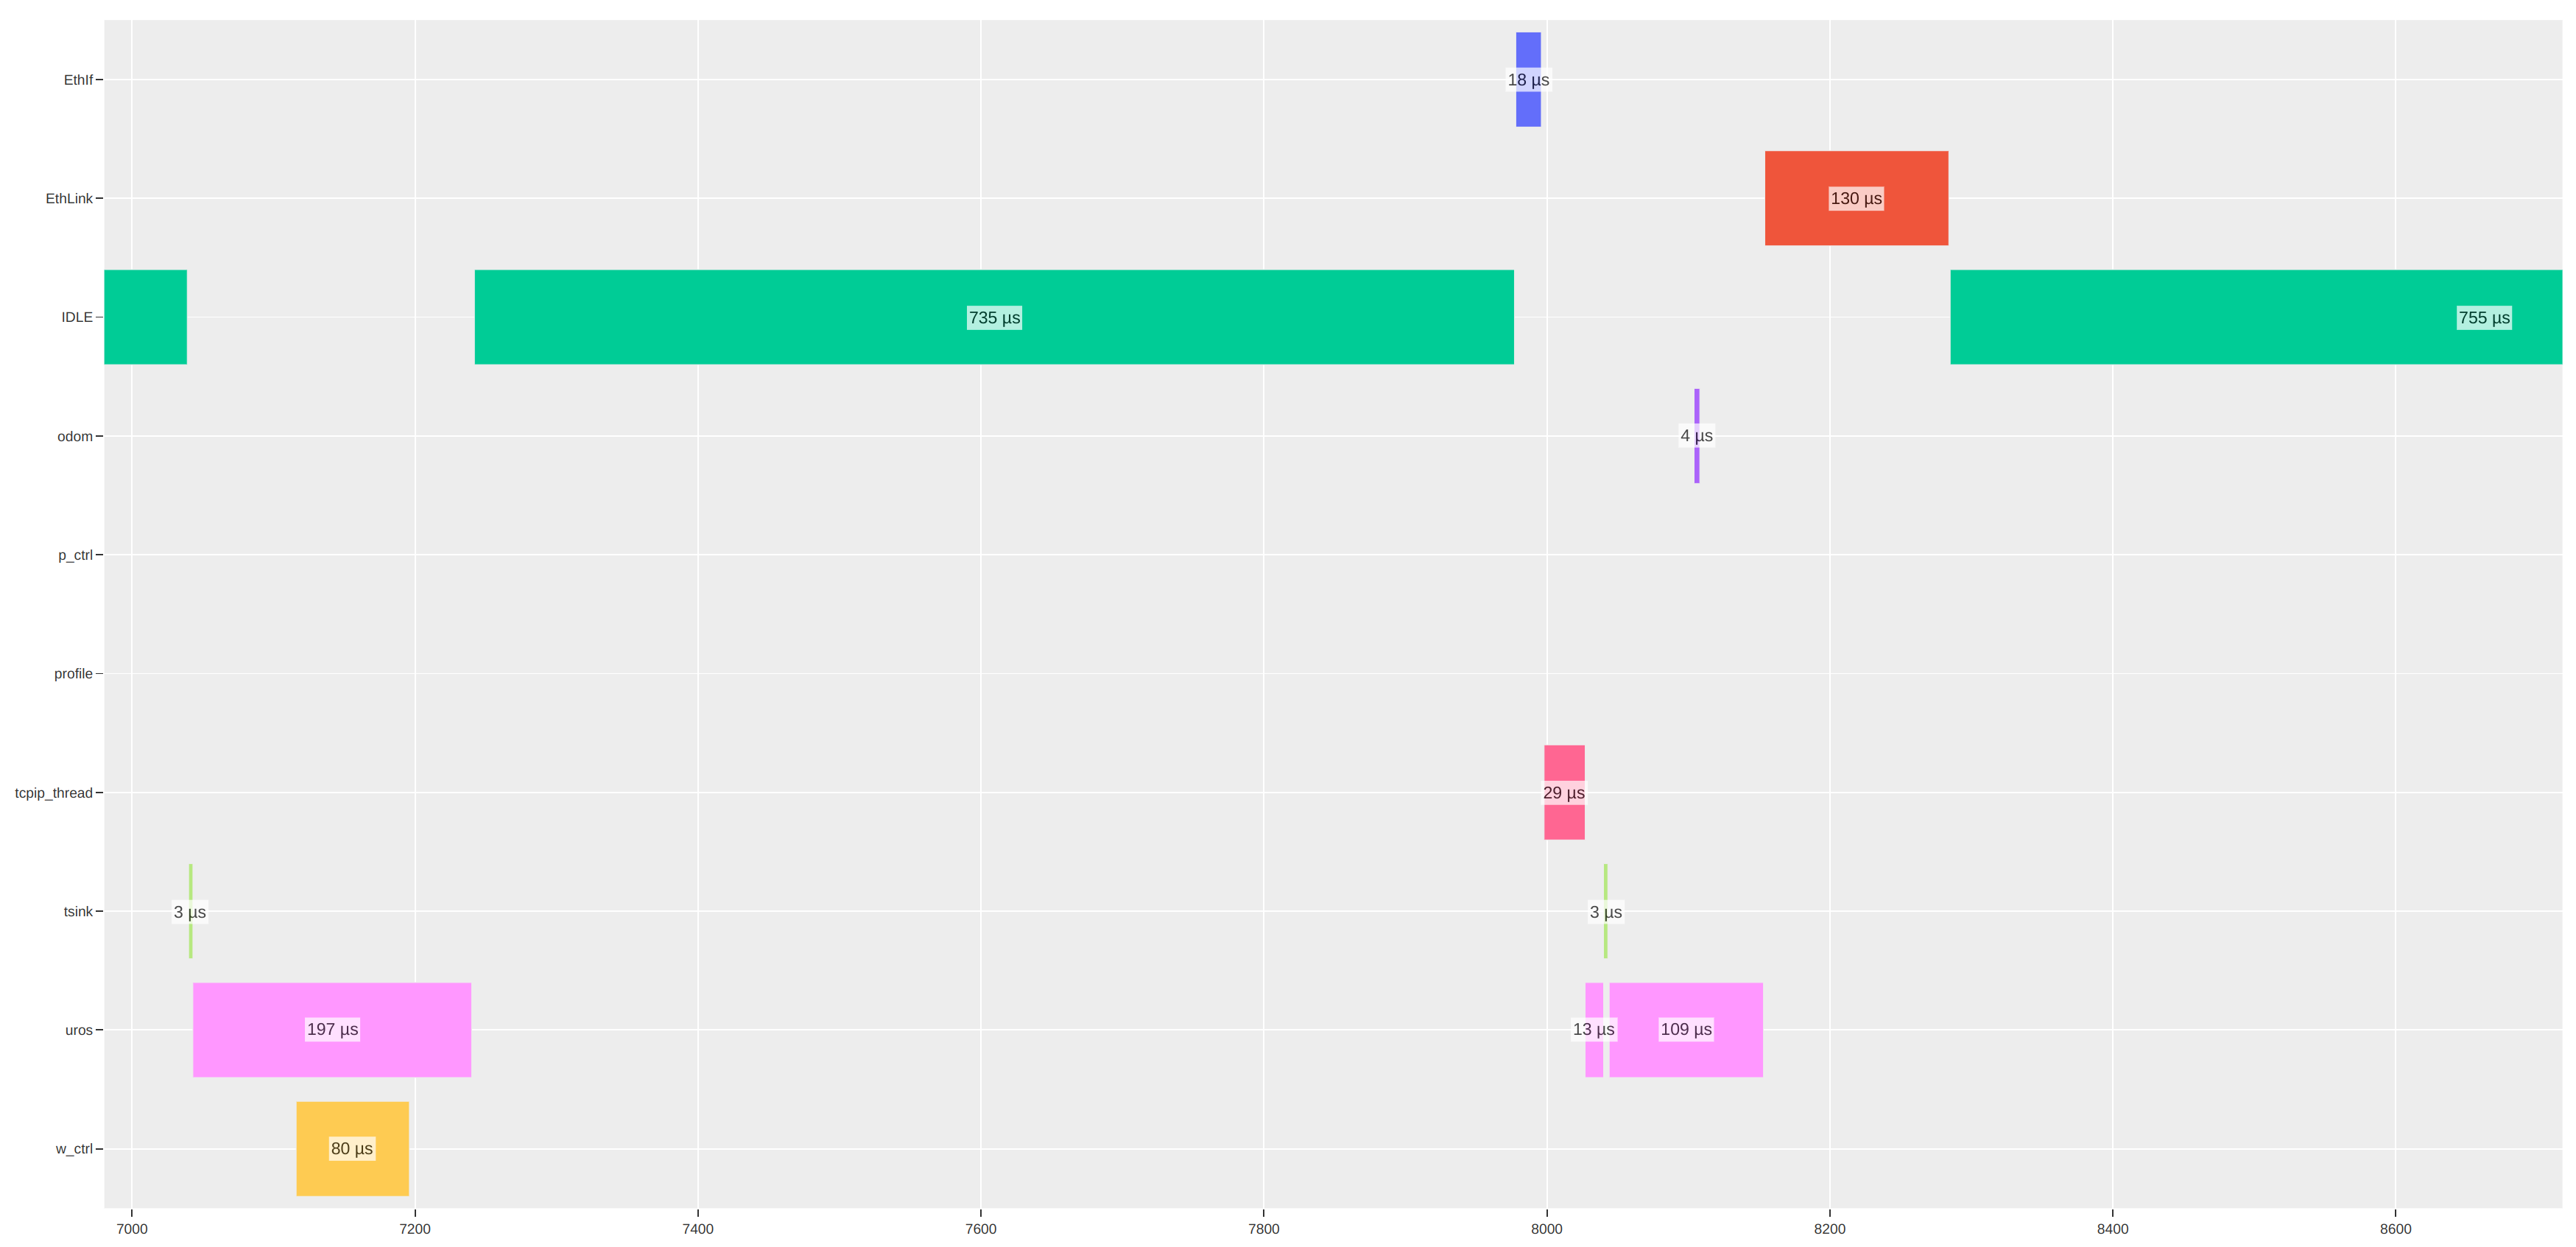
\includegraphics[width=1\textwidth]{assets/micro_ros_profiling_ausschnitt_cache_enabled}
    \caption{Echtzeitanalyse (Ausschnitt) unter Micro-ROS}
    % \label{fig:freertos_profiling}
\end{figure}

Die generierten profiling-daten reflektieren die echtzeitsaspekte bei dem
task-scheduling und den zeitkritischen funktionen. Ein Python-Skript
visualisiert diese Daten als Gantt-Diagramm, indem es die Start- und Endzeiten
mittels der \mintinline{text}|pandas| Bibliothek aggregiert, sortiert und dann
mittels der \mintinline{text}|Plotly| Bibliothek visualisiert ausgibt.

Am ende des Profilings wird eine Zusammenfassung durch von FreeRTOS
bereitgestellte \mintinline{cpp}|vTaskGetRunTimeStats()| und
\mintinline{cpp}|vTaskList()| ausgegeben.

\subsection{Laufzeit-Statistik -- Micro-ROS}

\subsubsection{Regler mit 50 Hz und 30 Hz}

Mit einer Sollfrequenz von $50\,\text{Hz}$ für die Drehzahlregelung und $30\,\text{Hz}$ für
die Posenregelung sowie Odometrie ergeben sich nach etwa $18$ Sekunden Profiling
folgende Messwerte:

\begin{table}[H]
\centering
\small
\setlength{\tabcolsep}{4pt}
\makebox[0pt][c]{\parbox{1.1\textwidth} \\ \hline
        \mintinline{text}|EthIf| & 52,93 & 115.022 & 0,62\,\% \\ \hline
        \mintinline{text}|EthLink| & 128,38 & 26.702 & 0,14\,\% \\ \hline
        \mintinline{text}|IDLE| & 587,79 & 8.961.378 & \textbf{48,17\,\%} \\ \hline
        \mintinline{text}|odom| & 8,88 & 8.186 & \textbf{0,04\,\%} \\ \hline
        \mintinline{text}|p_ctrl| & 277,97 & 170.671 & \textbf{0,92\,\%} \\ \hline
        \mintinline{text}|profile| & 623,40 & 4.981.587 & 26,78\,\% \\ \hline
        \mintinline{text}|tcpip_thread| & 71,16 & 176.607 & 0,95\,\% \\ \hline
        \mintinline{text}|tsink| & 8,80 & 120.659 & 0,65\,\% \\ \hline
        \mintinline{text}|uros| & 203,31 & 3.807.442 & \textbf{20,47\,\%} \\ \hline
        \mintinline{text}|w_ctrl| & 256,11 & 236.136 & \textbf{1,27\,\%} \\ \hline
        \hline
        \textbf{Summe} & - & 18.604.390 & 100,00\,\% \\ \hline
        \end{tabular}
        \caption{Laufzeit-Statistik ohne Caching}
    \end{minipage}
    \hfill
    \begin{minipage}[b]{0.50\hsize}\centering
        \begin{tabular}{|l|r|r|r|}
        \hline
        \textbf{Name}  & \textbf{Ø (µs)} & \textbf{Summe} & \textbf{\%} \\ \hline
        \mintinline{text}|EthIf| & 18,43 & 40.671 & 0,21\,\% \\ \hline
        \mintinline{text}|EthLink| & 123,53 & 24.583 & 0,13\,\% \\ \hline
        \mintinline{text}|IDLE| & 661,14 & 15.505.748 & \textbf{81,81\,\%} \\ \hline
        \mintinline{text}|odom| & 4,02 & 3.791 & \textbf{0,02\,\%} \\ \hline
        \mintinline{text}|p_ctrl| & 88,25 & 55.511 & \textbf{0,29\,\%} \\ \hline
        \mintinline{text}|profile| & 803,55 & 1.517.905 & 8,01\,\% \\ \hline
        \mintinline{text}|tcpip_thread| & 28,29 & 63.613 & 0,34\,\% \\ \hline
        \mintinline{text}|tsink| & 3,37 & 41.113 & 0,22\,\% \\ \hline
        \mintinline{text}|uros| & 76,17 & 1.614.854 & \textbf{8,52\,\%} \\ \hline
        \mintinline{text}|w_ctrl| & 90,82 & 85.646 & \textbf{0,45\,\%} \\ \hline
        \hline
        \textbf{Summe} & - & 18.953.435 & 100,00\,\% \\ \hline
        \end{tabular}
        \caption{Laufzeit-Statistik mit Caching}
    \end{minipage}
}}
\end{table}

\subsubsection{Regler mit 100 Hz und 50 Hz}

Mit einer Sollfrequenz von $100\,\text{Hz}$ für die Drehzahlregelung und $50\,\text{Hz}$ für
die Posenregelung sowie Odometrie ergeben sich nach etwa $18$ Sekunden Profiling
folgende Messwerte:

\begin{table}[H]
\centering
\small
\setlength{\tabcolsep}{4pt}
\makebox[0pt][c]{\parbox{1.1\textwidth} \\ \hline
        \mintinline{text}|EthIf| & 51,53 & 198.643 & 1,05\,\% \\ \hline
        \mintinline{text}|EthLink| & 110,25 & 26.130 & 0,14\,\% \\ \hline
        \mintinline{text}|IDLE| & 545,36 & 7.330.732 & \textbf{38,75\,\%} \\ \hline
        \mintinline{text}|odom| & 9,92 & 18.149 & \textbf{0,10\,\%} \\ \hline
        \mintinline{text}|p_ctrl| & 322,41 & 295.008 & \textbf{1,56\,\%} \\ \hline
        \mintinline{text}|profile| & 566,25 & 5.472.282 & 28,92\,\% \\ \hline
        \mintinline{text}|tcpip_thread| & 71,13 & 296.128 & 1,57\,\% \\ \hline
        \mintinline{text}|tsink| & 8,80 & 113.096 & 0,60\,\% \\ \hline
        \mintinline{text}|uros| & 231,74 & 4.606.256 & \textbf{24,35\,\%} \\ \hline
        \mintinline{text}|w_ctrl| & 307,53 & 562.785 & \textbf{2,97\,\%} \\ \hline
        \hline
        \textbf{Summe} & -- & 18.919.209 & 100,00\,\% \\ \hline
        \end{tabular}
        \caption{Laufzeit-Statistik ohne Caching}
    \end{minipage}
    \hfill
    \begin{minipage}[b]{0.50\hsize}\centering
        \begin{tabular}{|l|r|r|r|}
        \hline
        \textbf{Name}  & \textbf{Ø (µs)} & \textbf{Summe} & \textbf{\%} \\ \hline
        \mintinline{text}|EthIf| & 18,81 & 68.712 & 0,37\,\% \\ \hline
        \mintinline{text}|EthLink| & 128,88 & 23.971 & 0,13\,\% \\ \hline
        \mintinline{text}|IDLE| & 607,96 & 14.540.662 & \textbf{78,00\,\%} \\ \hline
        \mintinline{text}|odom| & 3,74 & 6.780 & \textbf{0,04\,\%} \\ \hline
        \mintinline{text}|p_ctrl| & 75,16 & 69.301 & \textbf{0,37\,\%} \\ \hline
        \mintinline{text}|profile| & 889,48 & 1.641.972 & 8,81\,\% \\ \hline
        \mintinline{text}|tcpip_thread| & 28,25 & 104.623 & 0,56\,\% \\ \hline
        \mintinline{text}|tsink| & 3,43 & 36.583 & 0,20\,\% \\ \hline
        \mintinline{text}|uros| & 86,44 & 1.957.616 & \textbf{10,50\,\%} \\ \hline
        \mintinline{text}|w_ctrl| & 103,59 & 191.027 & \textbf{1,02\,\%} \\ \hline
        \hline
        \textbf{Summe} & -- & 18.641.247 & 100,00\,\% \\ \hline
        \end{tabular}
        \caption{Laufzeit-Statistik mit Caching}
    \end{minipage}
}}
\end{table}

Ohne D- oder I-Cache benötigte die Micro-ROS-Task (\mintinline{text}|uros|) für
die gesamte Steuerungslogik bei den Reglern mit jeweils $50$ und $30\,\text{Hz}$
$\textbf{20,47\,\%}$ Rechenzeit, bzw. $\textbf{24,35\,\%}$ bei jeweils $100$ und
$50\,\text{Hz}$, während sich das System zu $\textbf{48,17\,\%}$ bzw.
$\textbf{38,75\,\%}$ im Leerlauf befindet.

Mit dem D- und I-Cache benötigt die Robotersteuerungslogik insgesamt nur
$\textbf{8,52\,\%}$ Rechenzeit bei den Reglern mit jeweils $50$ und
$30\,\text{Hz}$, oder $\textbf{10,50\,\%}$ bei jeweils $100$ und
$50\,\text{Hz}$, mit einer Leerlaufzeit von $\textbf{81,81\,\%}$ oder
$\textbf{78,00\,\%}.$

Durch das Aktivieren von Caches hat sich die akkumulierte Rechenzeit
beispielsweise bei der $100\,\text{Hz}|50\,\text{Hz}$ Regler-Konfiguration für
die Odometrie um $\textbf{62,64\,\%},$ für die Posenregelung um
$\textbf{76,51\,\%}$ sowie für die Drehzahlregelung um $\textbf{66,06\,\%}$
verringert, während die Leerlaufzeiten um $\textbf{98,35\,\%}$ erhöht wurden,
wobei sich die gesamten Profiling-Dauer mit einer Differenz von
$349,045\,\text{ms}$ unterscheiden.

\subsection{Laufzeit-Statistik -- FreeRTOS}

\subsubsection{Regler mit 50 Hz und 30 Hz}

\begin{table}[H]
\centering
\small
\setlength{\tabcolsep}{4pt}
\makebox[0pt][c]{\parbox{1.1\textwidth} \\ \hline
        \mintinline{text}|IDLE| & 983,50 & 14.996.422 & \textbf{81,85\%} \\ \hline
        \mintinline{text}|hal_fetch| & 21,71 & 20.403 & 0,11\% \\ \hline
        \mintinline{text}|odometry| & 24,05 & 13.634 & \textbf{0,07\%} \\ \hline
        \mintinline{text}|pose_control| & 32,66 & 18.682 & \textbf{0,10\%} \\ \hline
        \mintinline{text}|profile| & 902,87 & 3.077.879 & 16,80\% \\ \hline
        \mintinline{text}|tsink| & 9,63 & 161.451 & 0,88\% \\ \hline
        \mintinline{text}|wheel_ctrl| & 35,80 & 34.260 & \textbf{0,19\%} \\ \hline
        \hline
        \textbf{Summe} & -- & 18.322.731 & 100,00\,\% \\ \hline
        \end{tabular}
        \caption{Laufzeit-Statistik ohne Caching}
    \end{minipage}
    \hfill
    \begin{minipage}[b]{0.50\hsize}\centering
        \begin{tabular}{|l|r|r|r|}
        \hline
        \textbf{Name}  & \textbf{Ø (µs)} & \textbf{Summe} & \textbf{\%} \\ \hline
        \mintinline{text}|IDLE| & 1.041,06 & 17.658.382 & \textbf{94,83\,\%} \\ \hline
        \mintinline{text}|hal_fetch| & 6,43 & 6.003 & 0,03\,\% \\ \hline
        \mintinline{text}|odometry| & 7,19 & 4.068 & \textbf{0,02\,\%} \\ \hline
        \mintinline{text}|pose_control| & 9,64 & 5.456 & \textbf{0,03\,\%} \\ \hline
        \mintinline{text}|profile| & 476,43 & 889.027 & 4,77\,\% \\ \hline
        \mintinline{text}|tsink| & 2,95 & 46.947 & 0,25\,\% \\ \hline
        \mintinline{text}|wheel_ctrl| & 10,96 & 10.379 & \textbf{0,06\,\%} \\ \hline
        \hline
        \textbf{Summe} & -- & 18.620.262 & 100,00\,\% \\ \hline
        \end{tabular}
        \caption{Laufzeit-Statistik mit Caching}
    \end{minipage}
}}
\end{table}

\subsubsection{Regler mit 100 Hz und 50 Hz}

\begin{table}[H]
\centering
\small
\setlength{\tabcolsep}{4pt}
\makebox[0pt][c]{\parbox{1.1\textwidth} \\ \hline
        \mintinline{text}|IDLE| & 997,02 & 14.706.086 & \textbf{80,67\,\%} \\ \hline
        \mintinline{text}|hal_fetch| & 21,91 & 40.471 & 0,22\,\% \\ \hline
        \mintinline{text}|odometry| & 24,01 & 22.373 & \textbf{0,12\,\%} \\ \hline
        \mintinline{text}|pose_control| & 32,46 & 30.579 & \textbf{0,17\,\%} \\ \hline
        \mintinline{text}|profile| & 941,93 & 3.209.167 & 17,60\,\% \\ \hline
        \mintinline{text}|tsink| & 9,36 & 151.046 & 0,83\,\% \\ \hline
        \mintinline{text}|wheel_ctrl| & 37,77 & 70.285 & \textbf{0,39\,\%} \\ \hline
        \hline
        \textbf{Summe} & {--} & 18.230.007 & 100,00\,\% \\ \hline
        \end{tabular}
        \caption{Laufzeit-Statistik ohne Caching}
    \end{minipage}
    \hfill
    \begin{minipage}[b]{0.50\hsize}\centering
        \begin{tabular}{|l|r|r|r|}
        \hline
        \textbf{Name}  & \textbf{Ø (µs)} & \textbf{Summe} & \textbf{\%} \\ \hline
        \mintinline{text}|IDLE| & 1.139,87 & 17.276.974 & \textbf{94,61\,\%} \\ \hline
        \mintinline{text}|hal_fetch| & 6,61 & 12.104 & 0,07\,\% \\ \hline
        \mintinline{text}|odometry| & 6,84 & 6.256 & \textbf{0,03\,\%} \\ \hline
        \mintinline{text}|pose_control| & 9,88 & 9.043 & \textbf{0,05\,\%} \\ \hline
        \mintinline{text}|profile| & 487,57 & 892.246 & 4,89\,\% \\ \hline
        \mintinline{text}|tsink| & 3,01 & 45.597 & 0,25\,\% \\ \hline
        \mintinline{text}|wheel_ctrl| & 10,69 & 19.559 & \textbf{0,11\,\%} \\ \hline
        \hline
        \textbf{Summe} & {--} & 18.443.591 & 100.00\,\% \\ \hline
        \end{tabular}
        \caption{Laufzeit-Statistik mit Caching}
    \end{minipage}
}}
\end{table}

Ohne die Micro-ROS-Abhängigkeit erreicht das System bereits ohne Nutzung von
Caches eine Leerlaufzeit von circa $\textbf{80\,\%}$, und mit Nutzung von Caches
von circa $\textbf{95\,\%}$.

Die Performance-Steigerung durch das Aktivieren der Caches ist bei der
FreeRTOS-Implementierung ebenfalls signifikant, wobei sich die gesamten
Profiling-Dauer bei der $100\,\text{Hz}|50\,\text{Hz}$-Reglerkonfiguration um
$213,584\,\text{ms}$ unterscheiden. Die Leerlaufzeit stieg dadurch zwar nur um
$\textbf{14,88\,\%}$, jedoch verringerten sich die Rechenzeiten deutlich: für
die Odometrie um $\textbf{72,04\,\%}$, für die Posenregelung um
$\textbf{70,43\,\%}$ und für die Drehzahlregelung um $\textbf{72,17\,\%}$.

\subsection{Vergleich zwischen Micro-ROS und FreeRTOS}

% | name | unter Micro-ROS (µs) | unter FreeRTOS (µs) | Differenz (µs) |
% | Odometrie | 6.780 (Ø: 3,74) | 6.256 (Ø: 6,84) | -524 |
% | Posenregelung | 69.301 (Ø: 75,16) | 9043 (Ø: 9,88) | 60258 (Ø: 65,28) |
% | Drehzahlregelung |191.027 (Ø: 103,59) | 19.559 (Ø: 10,69) | 171468 (Ø: 92,90) |

Aus den Profiling-Daten lässt sich folgender Vergleich zwischen der Micro-ROS-
und FreeRTOS-Implementierung für die Robotersteuerung ableiten:

\begin{table}[h]
\centering
\begin{tabular}{|l|r|r|r|}
\hline
    \textbf{Name} & \textbf{Micro-ROS (\text{µs})} & \textbf{FreeRTOS (\text{µs})} & \textbf{Differenz (\text{µs})} \\ \hline
Odometrie & 6.780 (Ø:~3,74) & 6.256 (Ø:~6,84) & -524 \\ \hline
Posenregelung & 69.301 (Ø:~75,16) & 9.043 (Ø:~9,88) & 60.258 (Ø:~65,28) \\ \hline
Drehzahlregelung & 191.027 (Ø:~103,59) & 19.559 (Ø:~10,69) & 171.468 (Ø:~92,90) \\ \hline
\end{tabular}
\caption{Vergleich der Rechenzeiten zwischen Micro-ROS und FreeRTOS}
\end{table}

Die Implementierung bleibt auf beiden Plattformen größtenteils gleich, abgesehen
vom Datenaustausch. Bei Micro-ROS müssen die Daten zusätzlich in einer
dedizierten Struktur mit Metadaten -- unter anderem einem Header mit Zeitstempel
in Sekunden und Nanosekunden -- umgewandelt werden, was einen wesentlichen
Overhead im Vergleich zu FreeRTOS verursacht. Dort können die Daten als
einfache, array-ähnliche Struktur direkt in die Warteschlange kopiert und
extrahiert werden.

Zusätzlich unterscheidet sich die FreeRTOS-Implementierung von Micro-ROS
dadurch, dass die Drehzahldaten nicht direkt vom Drehzahlregler abgefragt und an
die Odometrie übergeben werden. Stattdessen übernimmt eine dedizierte
FreeRTOS-Task \mintinline{cpp}|hal_fetch| die Übertragung dieser Daten sowohl an
den Drehzahlregler als auch an die Odometrie. Dadurch wird ein Teil des
Overheads vom Drehzahlregler entkoppelt.

Zusammenfassend lässt sich feststellen, dass die Robotersteuerungslogik sowohl
unter Micro-ROS als auch unter FreeRTOS vergleichsweise wenig Rechenzeit
benötigt. Dies gilt selbst bei potenziell höheren Sollfrequenzen, sofern die
Daten gecacht sind und nicht bei jedem Zugriff aus dem RAM geladen werden
müssen, welcher wesentlich langsamer ist als der L1-Cache. Dank des
leistungsstarken Mikrocontrollers in Kombination mit Cache-Nutzung und
optimiertem Code befindet sich das System daher überwiegend im Leerlauf.
